\section{Anexos}

    \begin{tinytable}
        \begin{tabular}{|C{1.2cm}|p{2cm}|p{1.2cm}|p{1.5cm}|}
        \hline
            \multirow{2}{1cm}{Type Size (pts.)} & \multicolumn{3}{c|}{Apperance} \\ [10pt]\cline{2-4}
            & Regular & Bold & Italic\\\hline
            6 & Table superscripts &  & \\\hline
            8 & Section titles, references, tables, table names, table captions, figure captions, footnotes, text subscripts, and superscripts &  & \\\hline
            9 &  & Abstract, Index Terms & \\\hline
            10 & Authors affiliations, main text, equations, first letter in section titles &  & Subheading  \\\hline
            11 & Authors names &  & \\\hline
            12 & Paper title &  & \\\hline
        \end{tabular}
        \captionof{table}{This is a simple table}
    \end{tinytable}
    
    
    \begin{figure}[H]
        \centering
        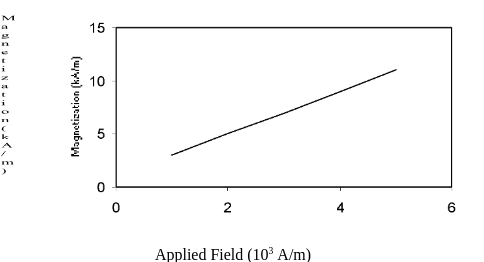
\includegraphics[width=0.9\linewidth]{images/imagen.png}
        \caption{Magnetization as a function of applied field. Note caption is centered below figures, but above tables.}
    \end{figure}